\section{Features of EEG data during sleep}

Contrary to the data used in the article \cite{vanPutten2018}, our challenge used EEG data recorded during the night. However, nocturnal brain rhythms present different caracteristics than diurnal ones. In this section, sleep spindles and K-complexes are studied : 
% TODO : decrire K complex
Sleep spindles are bursts of activity in the frequency range of 11-16 Hz and whose duration is 0.5 - 1.5 seconds. 
Note that the short duration of our EEG recordings makes it harder to efficiently detect sleep spindles, because the duration of latter is almost the same as our recordings. In other works, 10-seconds recordings are used.

\subsection{Brain rhythms}

The work studied in this challenge claimed Previous work such as \cite{Latta2005} showed evidence of a higher neural activity in the alpha and delta frequency range.

\subsection{Sleep spindles}

% TODO : parler des ondelettes https://raphaelvallat.com/spindles.html
% TODO : Presenter les sleep spindles. Parler de YASA et de la librairie de Dreem
% TODO : dire que les sleep spindles durent 0.5 - 1.5 seconde et que les echantillons durent 2 secondes, donc trop peu pour classifier efficacement les spindles

Several Python libraries are able to compute sleep spindles. In our work, we studied two of them : YASA\cite{Vallat2020} and Dosed\cite{Chambon2018}. These two libraries follow different approaches and are detailed below. 

\paragraph{YASA} This library is based on the work done in \cite{Lacourse2019} and detects sleep spindles using four well-chosen features : 
the absolute sigma power, the relative sigma power, the sigma covariance and the sigma correlation.
Applying this algorithm on the 264880 2-seconds recordings of our training set, 441 sleep spindles were detected. Figure (\ref{fig:spindles}) shows two examples of sleep spindles present in the training dataset. 

\begin{figure}
	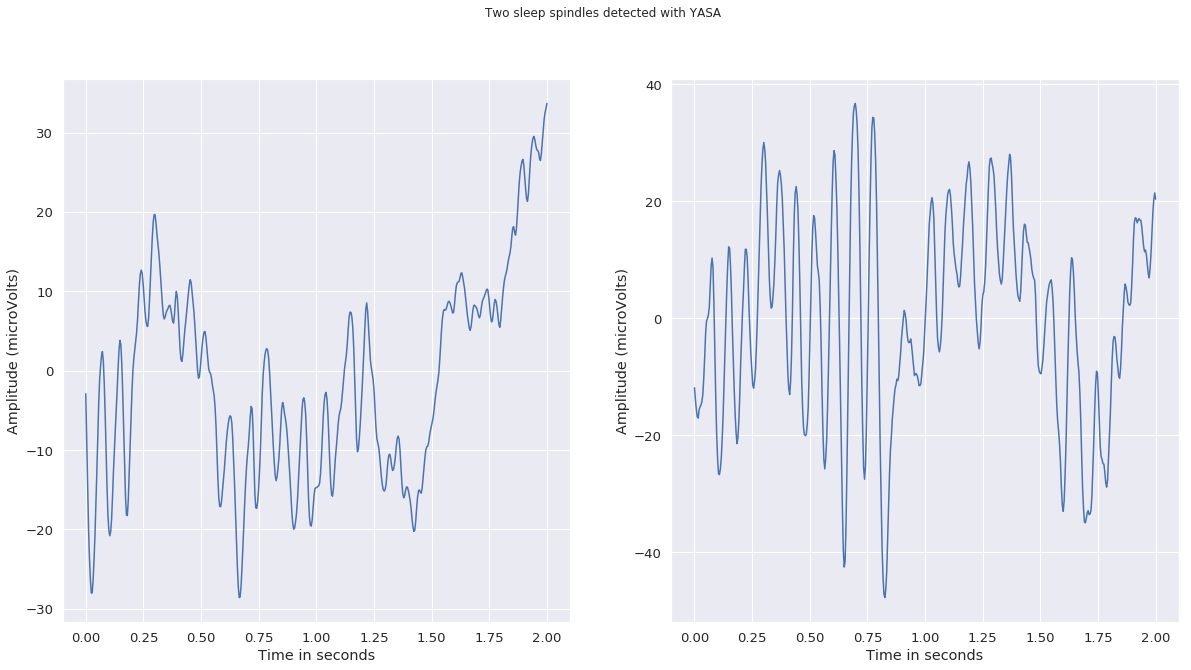
\includegraphics[width=\textwidth]{images/spindles_example.png}
	\caption{Example of two recordings showing sleep spindles, from revised x\_train.h5 file. Left : subject 1, sample 12, channel 4. Right : subject 3, sample 16, channel 5. We can clearly observe the oscillatory behavior lasting for about half a second.}
	\label{fig:spindles}
\end{figure}

% TODO :  echantillons, ou des parametres a tuner. 
% TODO : bla bla bla 

\paragraph{Dosed} Contrary to YASA, this Python library trains a deep learning model to identify sleep spindles. It thus requires training using annoted recordings where sleep spindles are already identified.
Because of our lack of time, we limiteed ourselves to YASA for our experiments, as it does not require supplementary data for training and was overall easier to use in our own codebase. 

\subsection{K-complexes}

\subsection{Correlation between sensors}
\label{sensor_correlations}

Observing the data leads us to observe a strong correlation between some channels : indeed, the pairs of channels (1, 5), (2, 6) and (3, 4) seem to show strongly correlated signals. To verify this fact, we computed a correlation matrix $M$ for each of the 946 $\times$ 40 recordings : the 7 $\times$ 7 matrix $M$ stores the value returned by the \texttt{numpy} function \texttt{np.correlate}($s_i$, $s_j$) for the signals of two sensors $s_i$, $s_j$. In our case, this function simply returns the cross product of the 500 dimensional vectors corresponding to each sensor. Then, for each row $i$ of M, we simply compute the sensor $j$ that maximizes the cross product with $i$ (other than $i$ itself). Doing this for all the recordings, we confirm the observation stated above. 

